\begin{enumerate}[\Large\bfseries 1.]

%--------------------1.
\item \textbf{\large Desigualdades que relacionan distintos tipos de promedios}\\\\

    \begin{enumerate}[\bfseries a)]

	%----------a.
	\item \textbf{(Tom Apostol, Calculus Vol 1)} Sean $x_1,x_2,...,x_n$ $n$ números reales positivos. Si $p$ es un entero no nulo, la media de potencias p-énesimas $M_p$ se define como sigue.
$$M_p = \left( \dfrac{x_1^{p} + ... + x_{n}^{p}}{n} \right)^{1/p}$$
El número $M_1$ se denomina media aritmética, $M_2$ media cuadrática y $M_{-1}$ media armónica.\\\\

	%----------b)
	\item \textbf{Código fuente.}\\ 
	    
	    \lstinputlisting[language=Python]{python/tareas_mat/week3/promedios.py}
	    \vspace{1cm}
	
	%----------c)
	\item \textbf{Prueba de la ejecución del programa}.\\
	    \begin{center}
		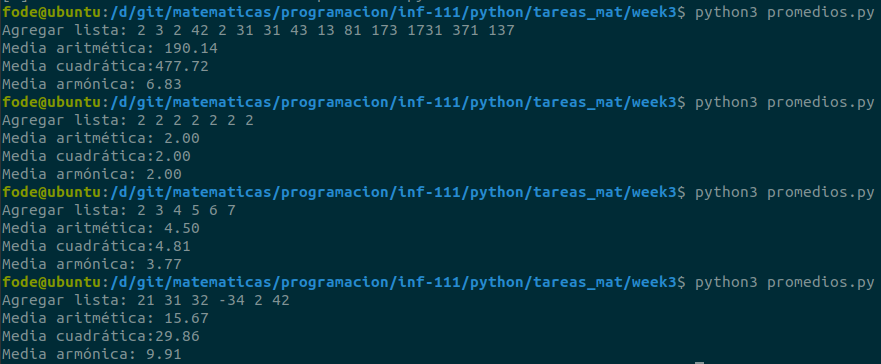
\includegraphics[scale=.42]{imagenes/tareas_mat/week3/promedios.png}
	    \end{center}

    \end{enumerate}

\newpage

%--------------------2.
\item

    \begin{enumerate}[\bfseries a)]

	%----------a.
	\item

	%----------b)
	\item \textbf{Código fuente.}\\ 
	    
	    \lstinputlisting[language=Python]{python/tareas_mat/week2/coe_binom.py}
	    \vspace{3cm}
	
	%----------c)
	\item \textbf{Prueba de la ejecución del programa}.\\
	    \begin{center}
		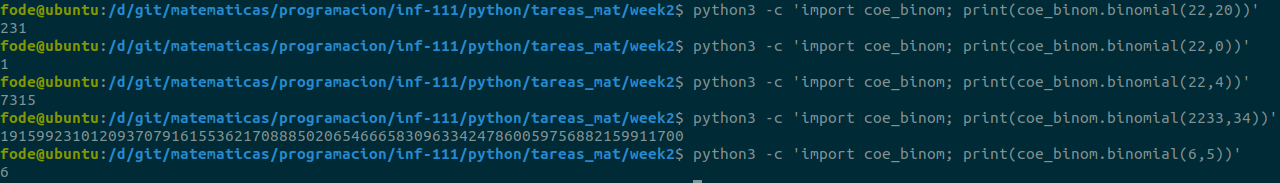
\includegraphics[scale=.35]{imagenes/tareas_mat/week2/coe_binom.png}
	    \end{center}

    \end{enumerate}

\newpage

%--------------------3.
\item

    \begin{enumerate}[\bfseries a)]

	%----------a.
	\item

	%----------b)
	\item \textbf{Código fuente.}\\ 
	    
	    \lstinputlisting[language=Python]{python/tareas_mat/week2/coe_binom.py}
	    \vspace{3cm}
	
	%----------c)
	\item \textbf{Prueba de la ejecución del programa}.\\
	    \begin{center}
		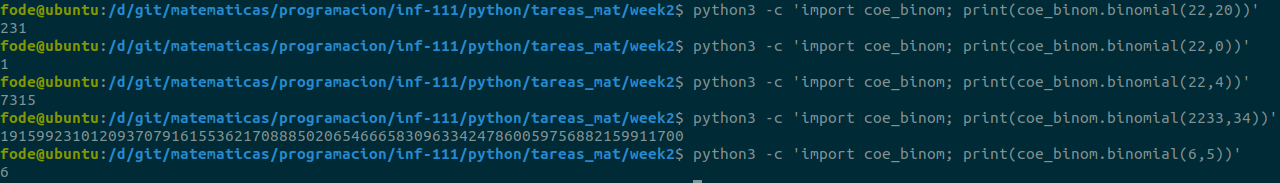
\includegraphics[scale=.35]{imagenes/tareas_mat/week2/coe_binom.png}
	    \end{center}

    \end{enumerate}

\newpage

%--------------------4.
\item

    \begin{enumerate}[\bfseries a)]

	%----------a.
	\item

	%----------b)
	\item \textbf{Código fuente.}\\ 
	    
	    \lstinputlisting[language=Python]{python/tareas_mat/week2/coe_binom.py}
	    \vspace{3cm}
	
	%----------c)
	\item \textbf{Prueba de la ejecución del programa}.\\
	    \begin{center}
		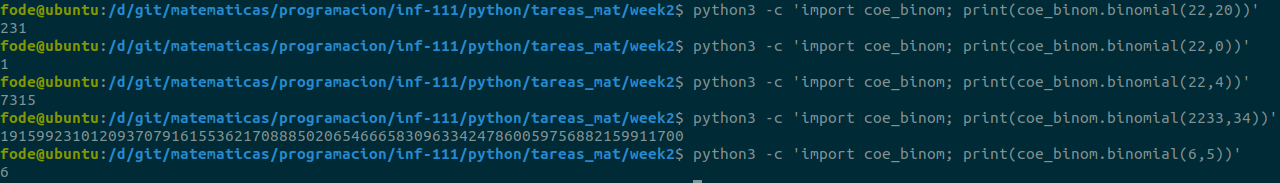
\includegraphics[scale=.35]{imagenes/tareas_mat/week2/coe_binom.png}
	    \end{center}

    \end{enumerate}

\newpage

%--------------------5.
\item

    \begin{enumerate}[\bfseries a)]

	%----------a.
	\item

	%----------b)
	\item \textbf{Código fuente.}\\ 
	    
	    \lstinputlisting[language=Python]{python/tareas_mat/week2/coe_binom.py}
	    \vspace{3cm}
	
	%----------c)
	\item \textbf{Prueba de la ejecución del programa}.\\
	    \begin{center}
		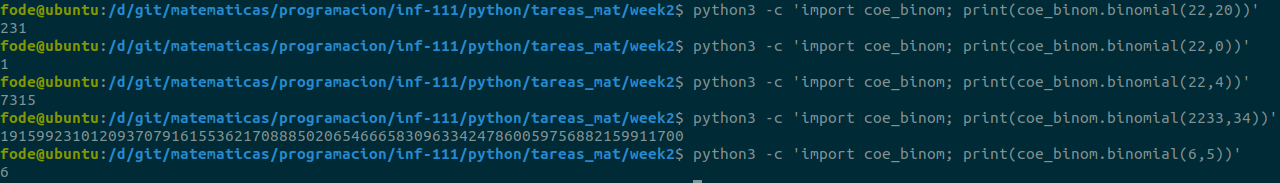
\includegraphics[scale=.35]{imagenes/tareas_mat/week2/coe_binom.png}
	    \end{center}

    \end{enumerate}

\newpage
\end{enumerate}
